%!TEX root = ../bericht.tex

\section{Einleitung}

eee

\section{Methoden}


	\subsection{Konzept}
	
		In der Entwicklung einer Osteosyntheseplatte sollen unterschiedliche Aspekte.
		Darunter fallen folgende Aspekte:
		
		\begin{enumerate}
			\setlength{\itemsep}{0mm}
			\setlength{\parskip}{1mm}
			\item Möglichst Minimal-Invasive Technik um Weichteile nicht zu verletzen
		\end{enumerate}
		
		Da meine CAD Konstruktions-Fähigkeiten beschränkt sind 	
		

\section{CAD Modellierung}

\section{FEM Analyse}

	\subsection{Materialdaten}
		\begin{center}
			\begin{tabular}{ | p{6cm} | p{3cm} | }
				\multicolumn{1}{l}{\bfseries Material} & \multicolumn{1}{l}{\bfseries E-Modus } \\ \hline
				Knochen (bone) & $ 1300 \frac{kg}{m^3} $ \\ \hline
				Titanlegierung (titanium alloy) & $ 4620 \frac{kg}{m^3} $ \\ \hline
			\end{tabular}
			\captionof{table}{Materialdaten}
			\label{fig:device3}
		\end{center}

	\subsection{Vernetzung}
		\begin{Figure}
			\centering
			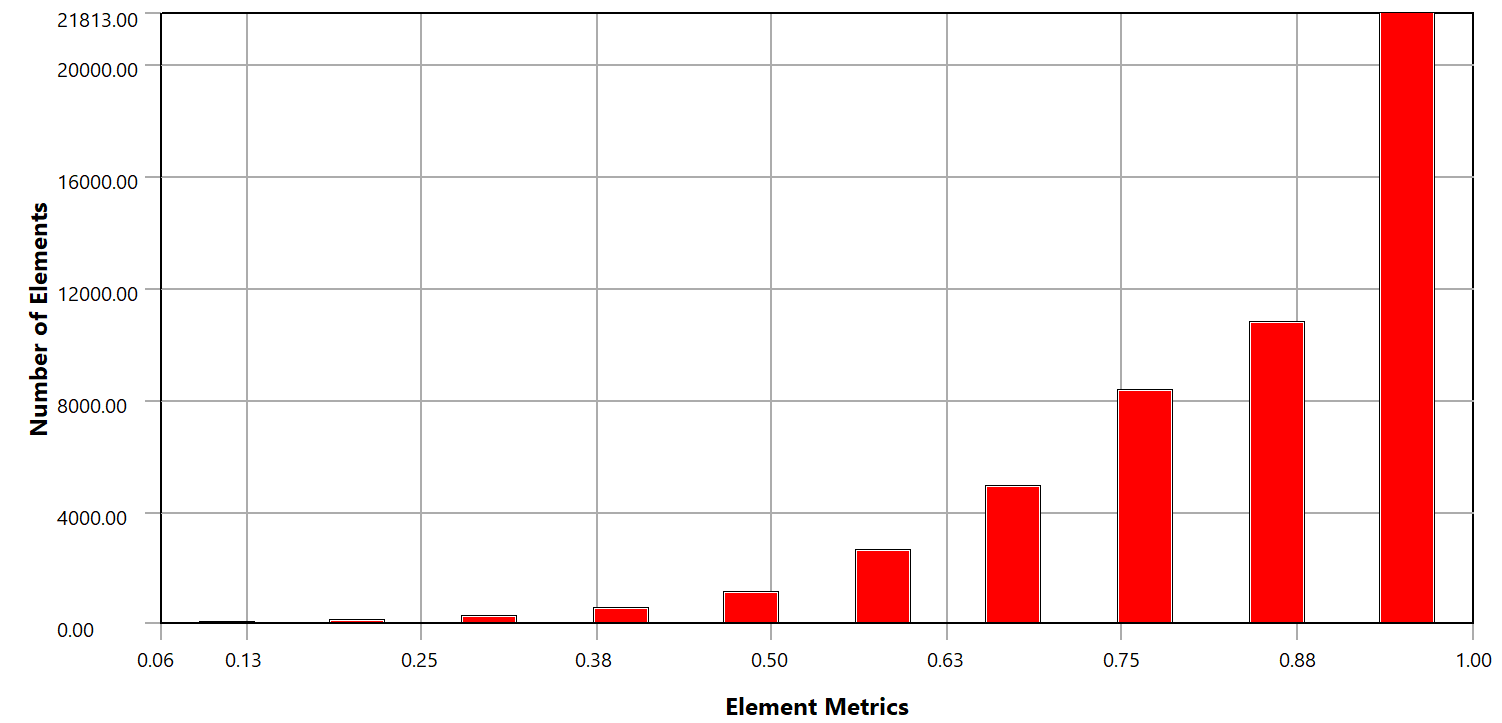
\includegraphics[width=15cm]{content/images/mesh_quality.png}
			\captionof{figure}{Magic-Angle-Spinning (MAS) Aufbau}
			\label{fig:device3}
		\end{Figure}
		
		\begin{Figure}
			\centering
			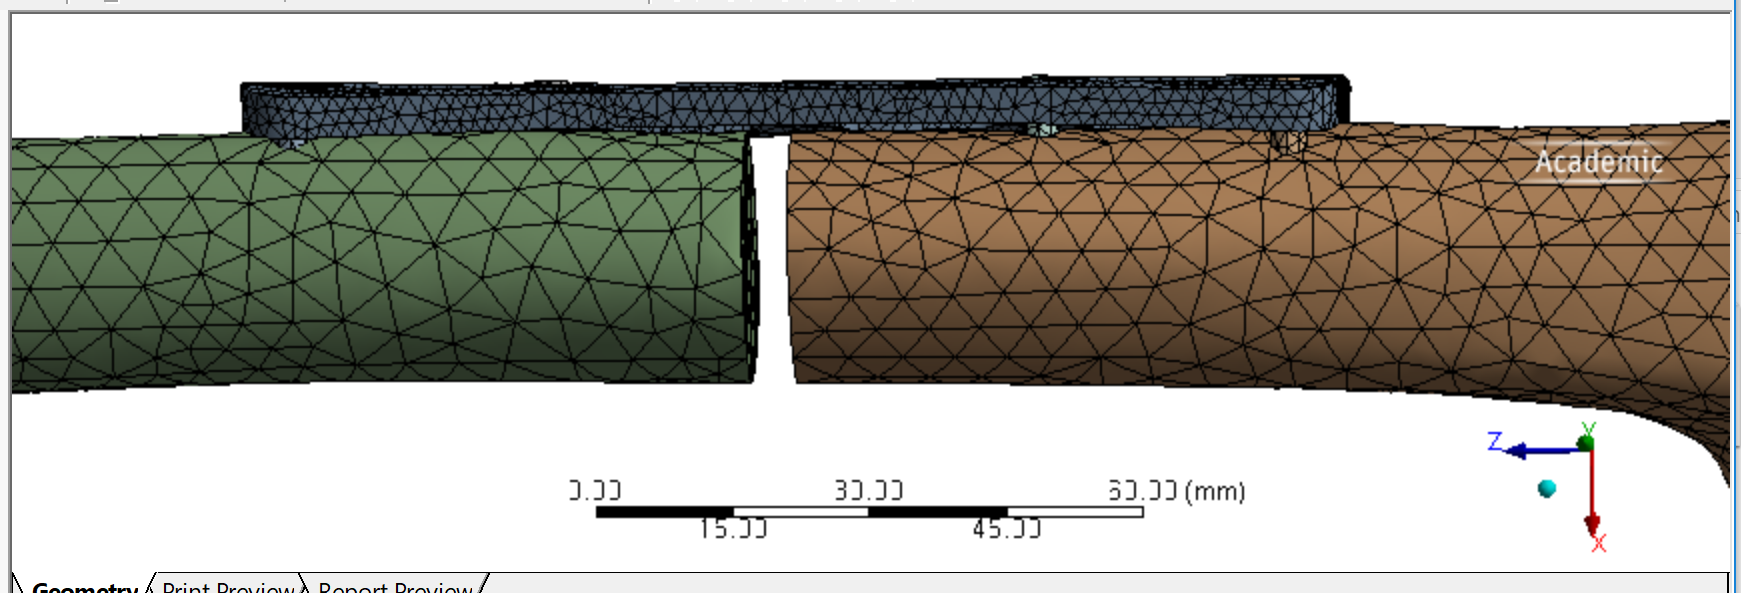
\includegraphics[width=15cm]{content/images/mesh_quality_graph_2.png}
			\captionof{figure}{Magic-Angle-Spinning (MAS) Aufbau}
			\label{fig:device3}
		\end{Figure}
		
		\begin{Figure}
			\centering
			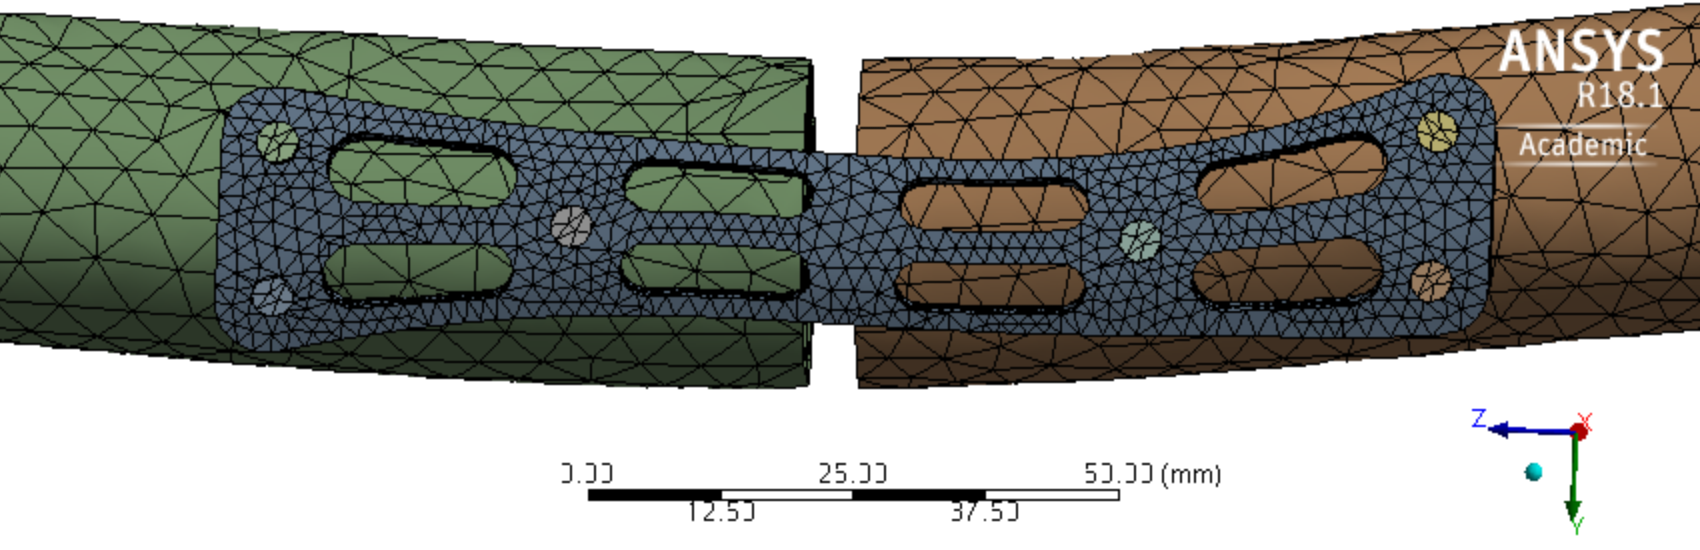
\includegraphics[width=15cm]{content/images/mesh_quality_graph_3.png}
			\captionof{figure}{Magic-Angle-Spinning (MAS) Aufbau}
			\label{fig:device3}
		\end{Figure}

	\subsection{Lager- und Reaktionskräfte}
		\begin{Figure}
			\centering
			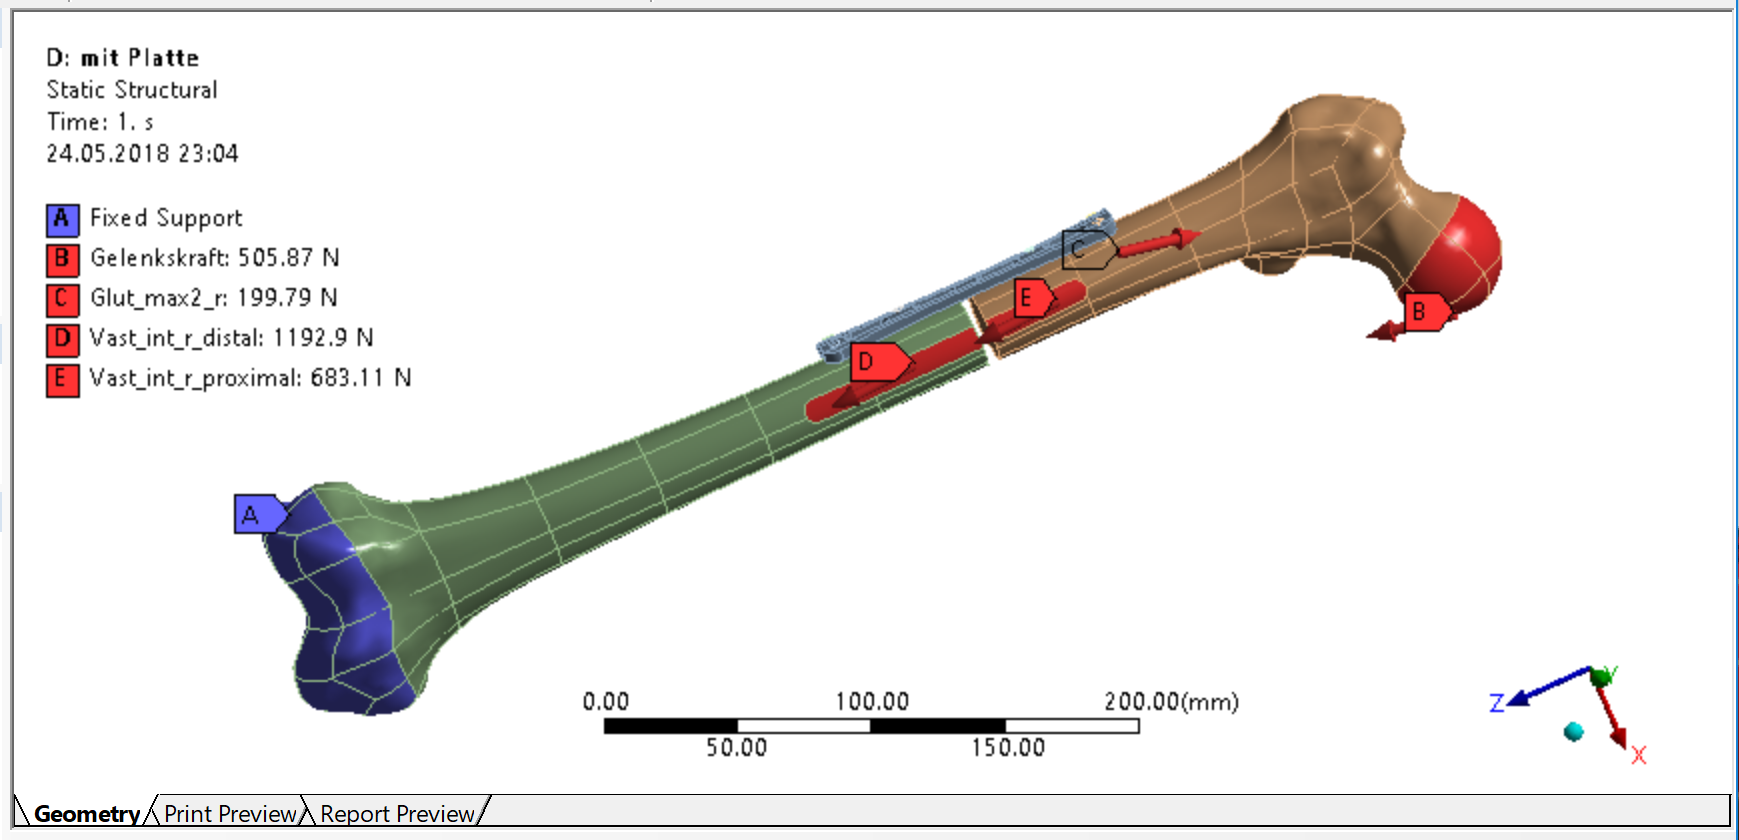
\includegraphics[width=15cm]{content/images/kraefte.png}
			\captionof{figure}{Magic-Angle-Spinning (MAS) Aufbau}
			\label{fig:device3}
		\end{Figure}


\section{Resultate}

	\subsection{Gesamtverformung}
	
		\begin{Figure}
			\centering
			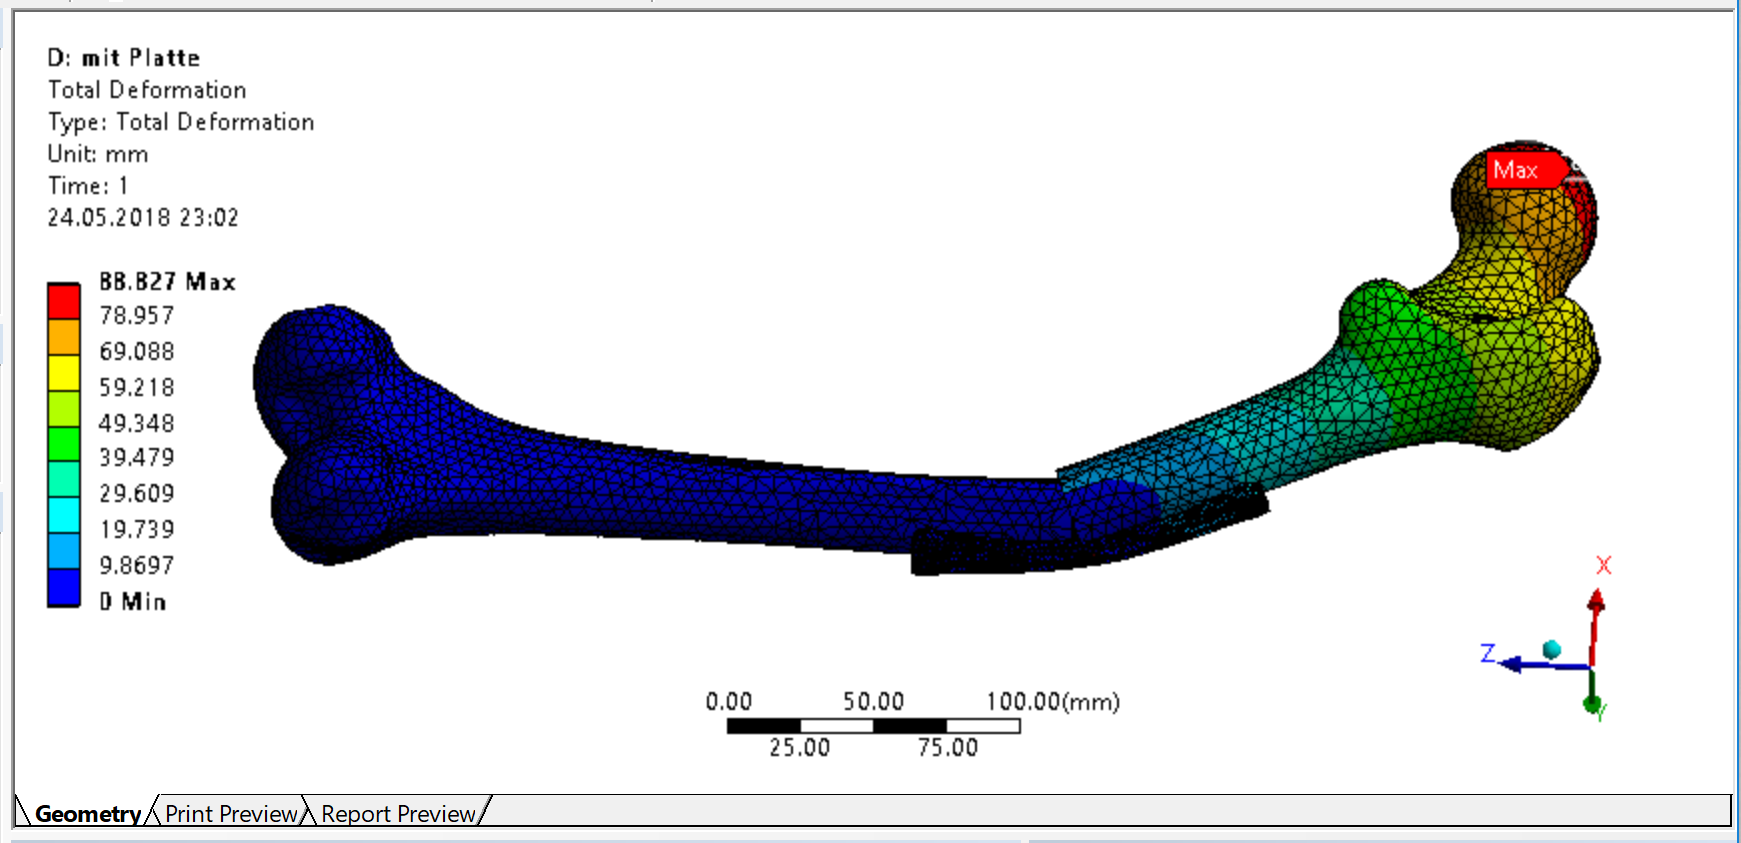
\includegraphics[width=15cm]{content/images/deformation.png}
				\captionof{figure}{Gesamtdeformation der Osteosyntheseplatte}
			\label{fig:deformation}
		\end{Figure}
	
		\subsubsection{Vergleichsplatte}
	
			\begin{Figure}
				\centering
				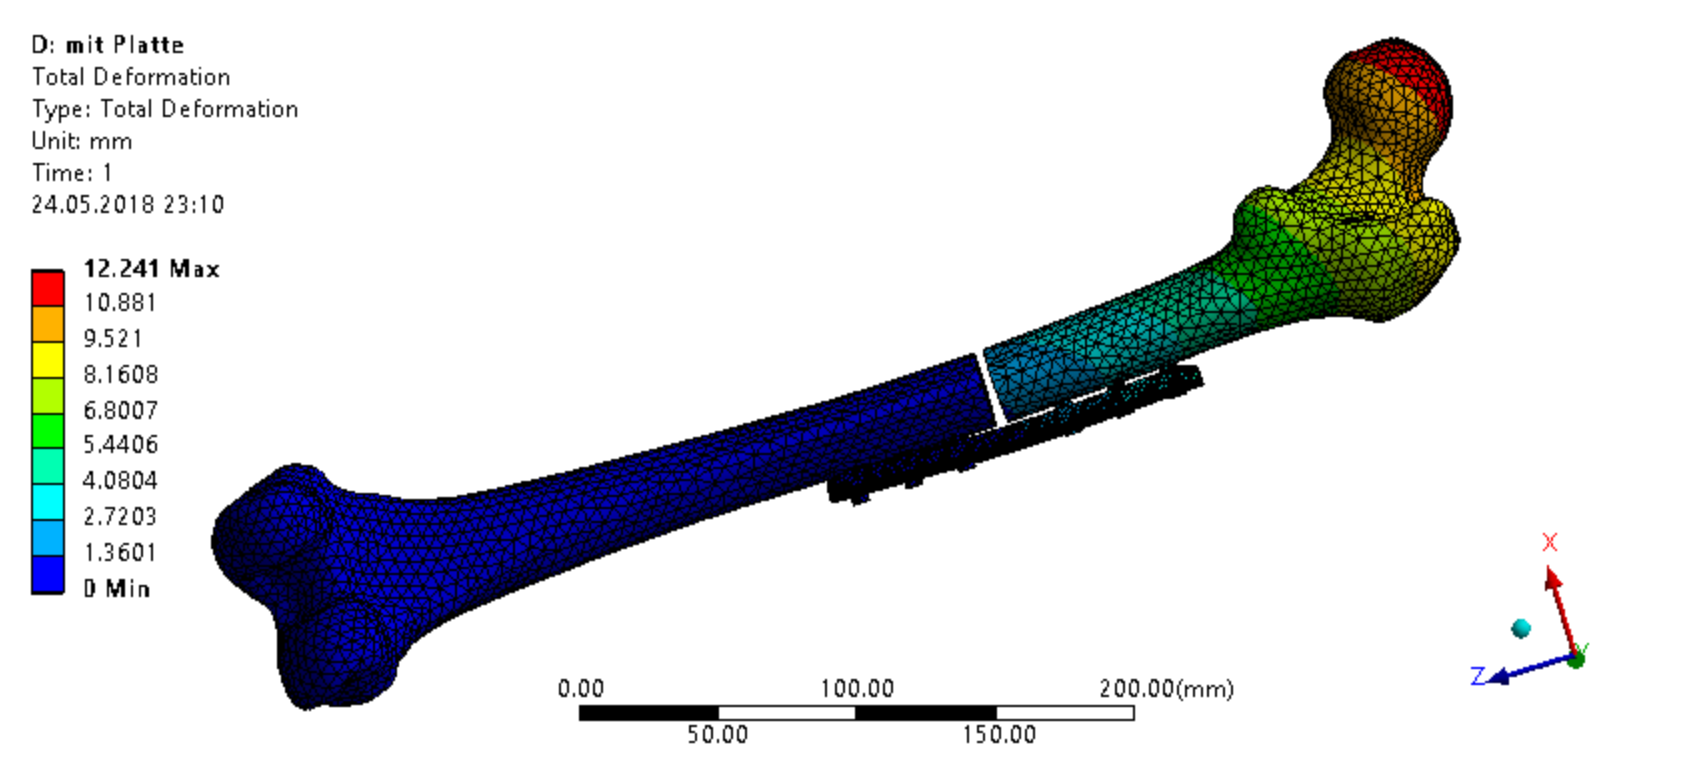
\includegraphics[width=15cm]{content/images/vergleich_deformation.png}
				\captionof{figure}{Gesamtdeformation der Vergleichsplatte}
				\label{fig:vergleich_deformation}
			\end{Figure}
	
	\subsection{Vergleichsspannung}
	
		\begin{Figure}
			\centering
			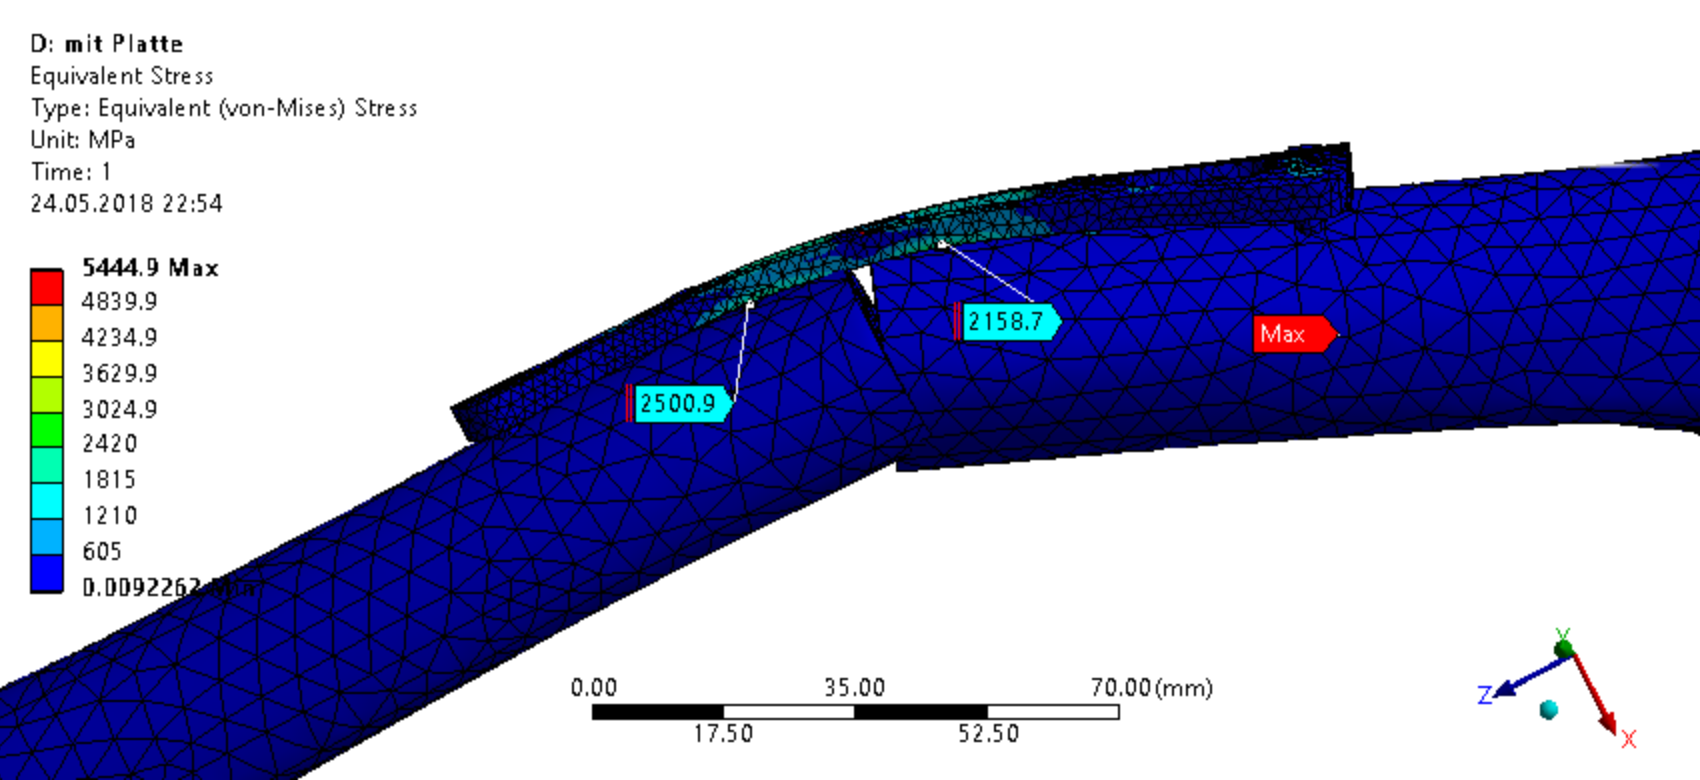
\includegraphics[width=15cm]{content/images/stress_side.png}
			\captionof{figure}{Vergleichsspannung der Osteosyntheseplatte (vorne)}
			\label{fig:stress_side}
		\end{Figure}
	
		\begin{Figure}
			\centering
			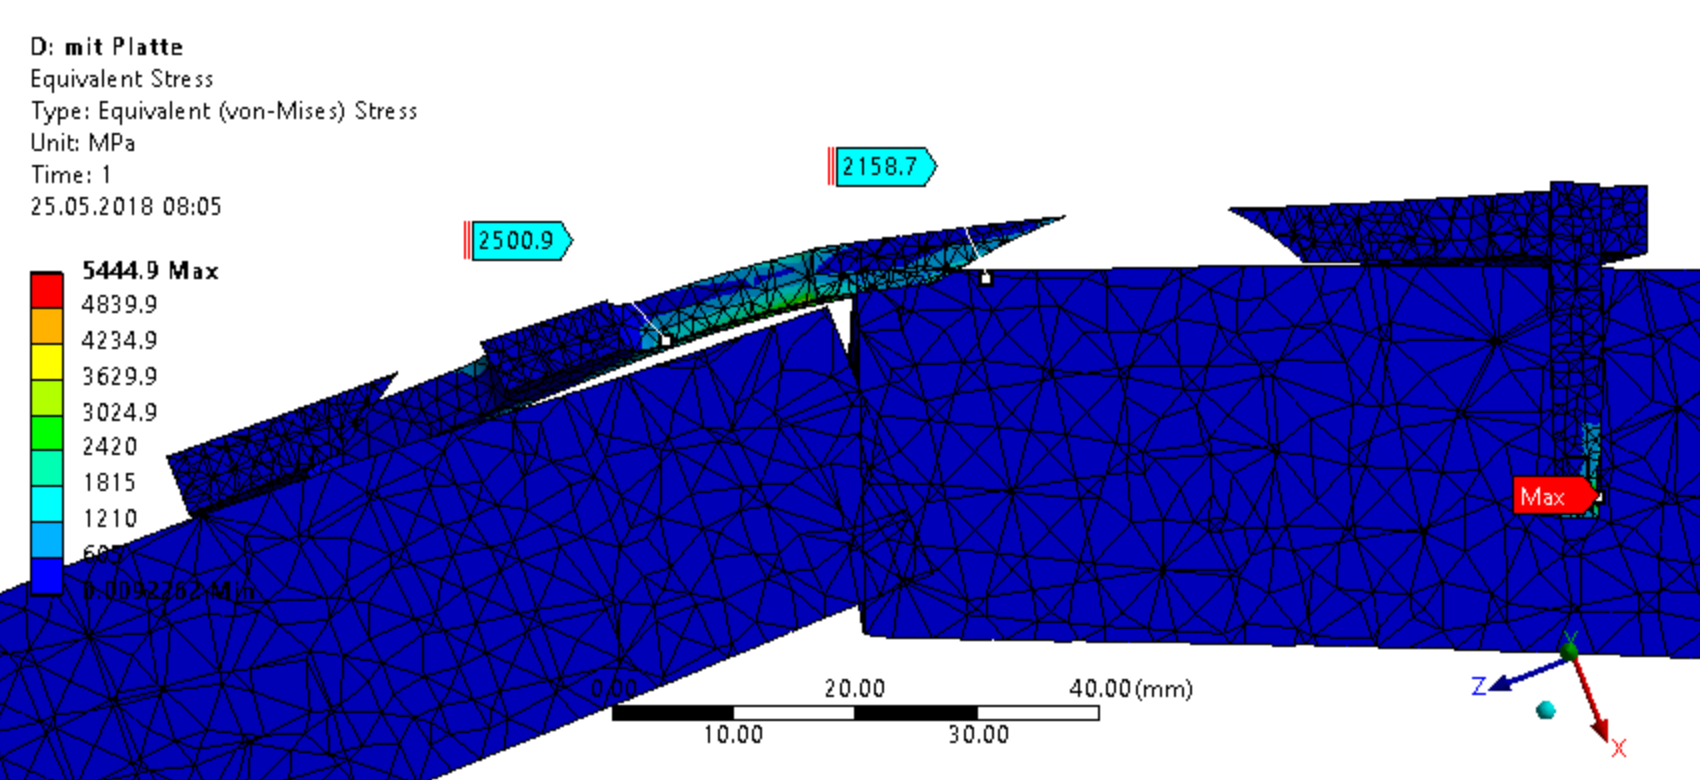
\includegraphics[width=15cm]{content/images/stress_side_profile.png}
			\captionof{figure}{Vergleichsspannung der Osteosyntheseplatte (vorne, im Querschnitt)}
			\label{fig:stress_side_profile}
		\end{Figure}
	
		\begin{Figure}
			\centering
			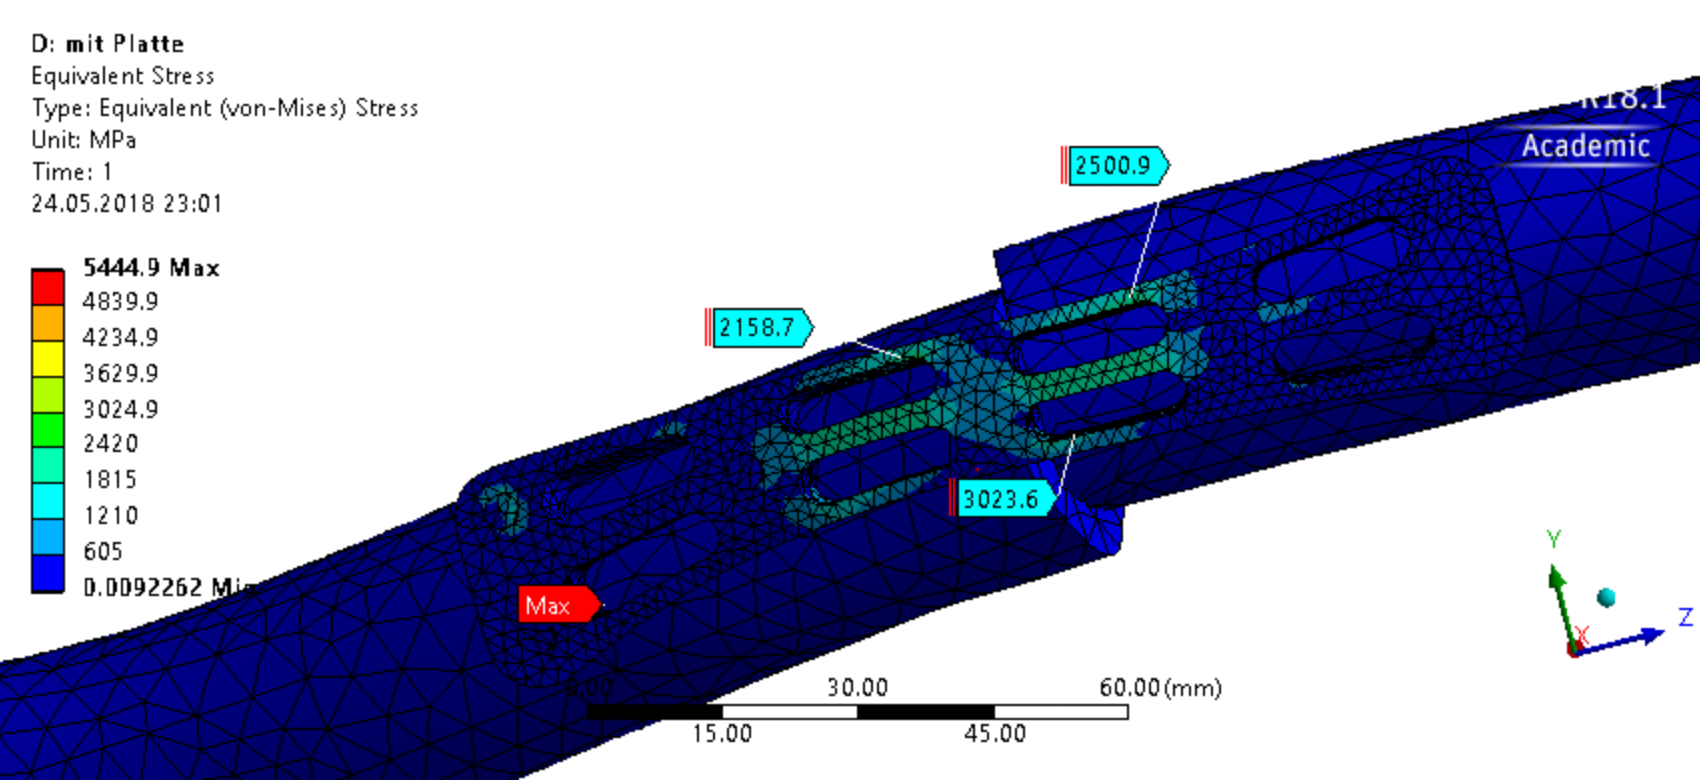
\includegraphics[width=15cm]{content/images/stress_top.png}
			\captionof{figure}{Vergleichsspannung der Osteosyntheseplatte (oben)}
			\label{fig:stress_top}
		\end{Figure}
		
		\subsubsection{Vergleichsplatte}
		
			\begin{Figure}
				\centering
				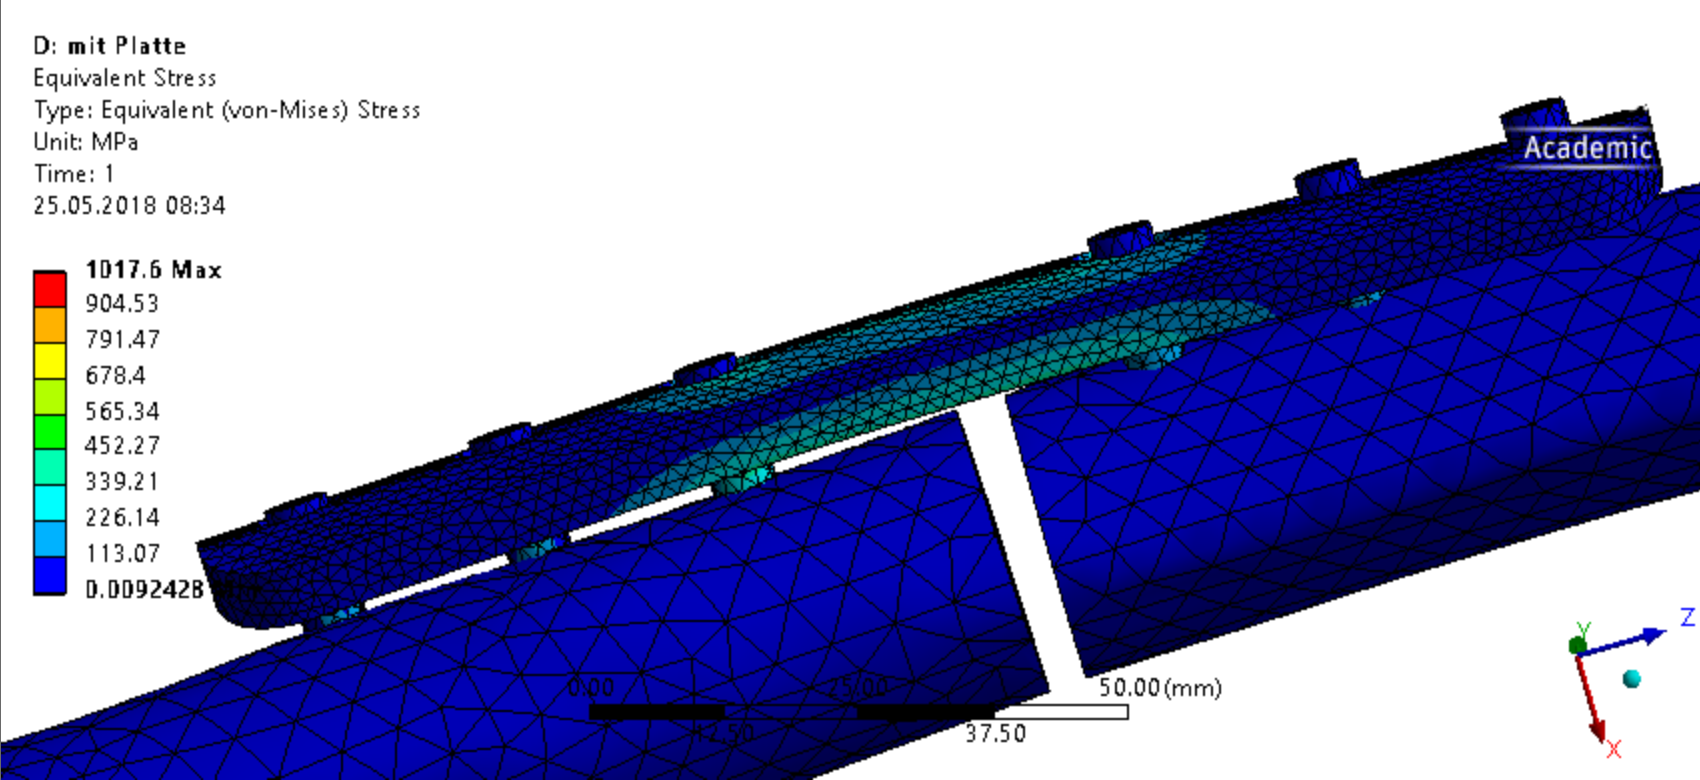
\includegraphics[width=15cm]{content/images/vergleich_stress_side.png}
				\captionof{figure}{Vergleichsspannung der Vergleichsplatte (vorne)}
				\label{fig:vergleich_stress_side}
			\end{Figure}
		
			\begin{Figure}
				\centering
				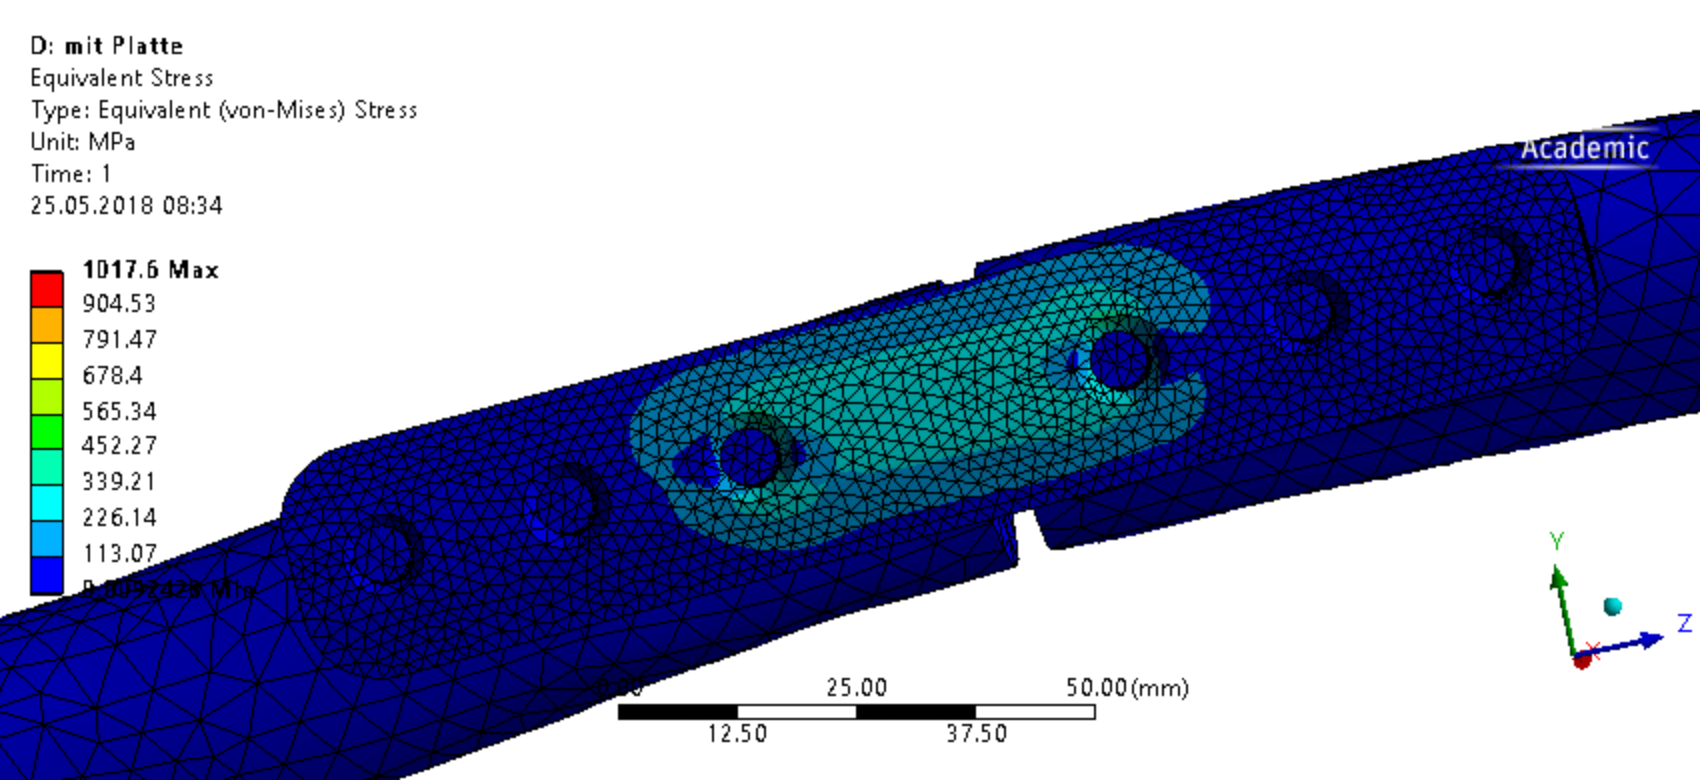
\includegraphics[width=15cm]{content/images/vergleich_stress_top.png}
				\captionof{figure}{Vergleichsspannung der Vergleichsplatte (oben)}
				\label{fig:vergleich_stress_top}
			\end{Figure}
	
	
	\subsection{Gegenüberstellung zwischen den Platten}
	
		Die Gegenüberstellung zwischen der neuen Osteosyntheseplatte und der Vergleichsplatte zeigt,
		dass die neue OSP in der Gesamtdeformation mit $ \SI{88.8}{mm} $ um ein Faktor von $ \SI{7}{} $
		grösser ist	gegenüber der Vergleichsplatte mit $ \SI{12.2}{mm} $.
		
		Auch die Vergleichsspannung der neuen OSP ist mit $ \SI{5444.9}{MPa} $ um ein Faktor von $ \SI{5}{} $
		grösser als die Vergleichsplatte mit $ \SI{10.176}{MPa} $.
	
	\subsection{Plausibilitätsrechnung}
		Für die Berechnung der Durchbiegung $w\left(l\right)$ wird das Flächenträgheitsmoment $I_{y}$ benötigt.
		Ein Röhrenknochen, wie im gegebenen Fall der Femur, besteht im Querschnitt aus \textit{Compacta},
		\textit{Spongiosa} und einer \textit{Markhöhlen}. 
		
		\begin{mycapequ}[!ht]
			\begin{align*}
				a\left(x\right) \cdot y\mkern3mu' + b\left(x\right) \cdot y & = g\left(x\right)
			\end{align*}
		\end{mycapequ}
	
		\begin{Figure}
			\centering
			\begin{tikzpicture}
				\node[anchor=south west,inner sep=0] at (0cm,0cm) {
					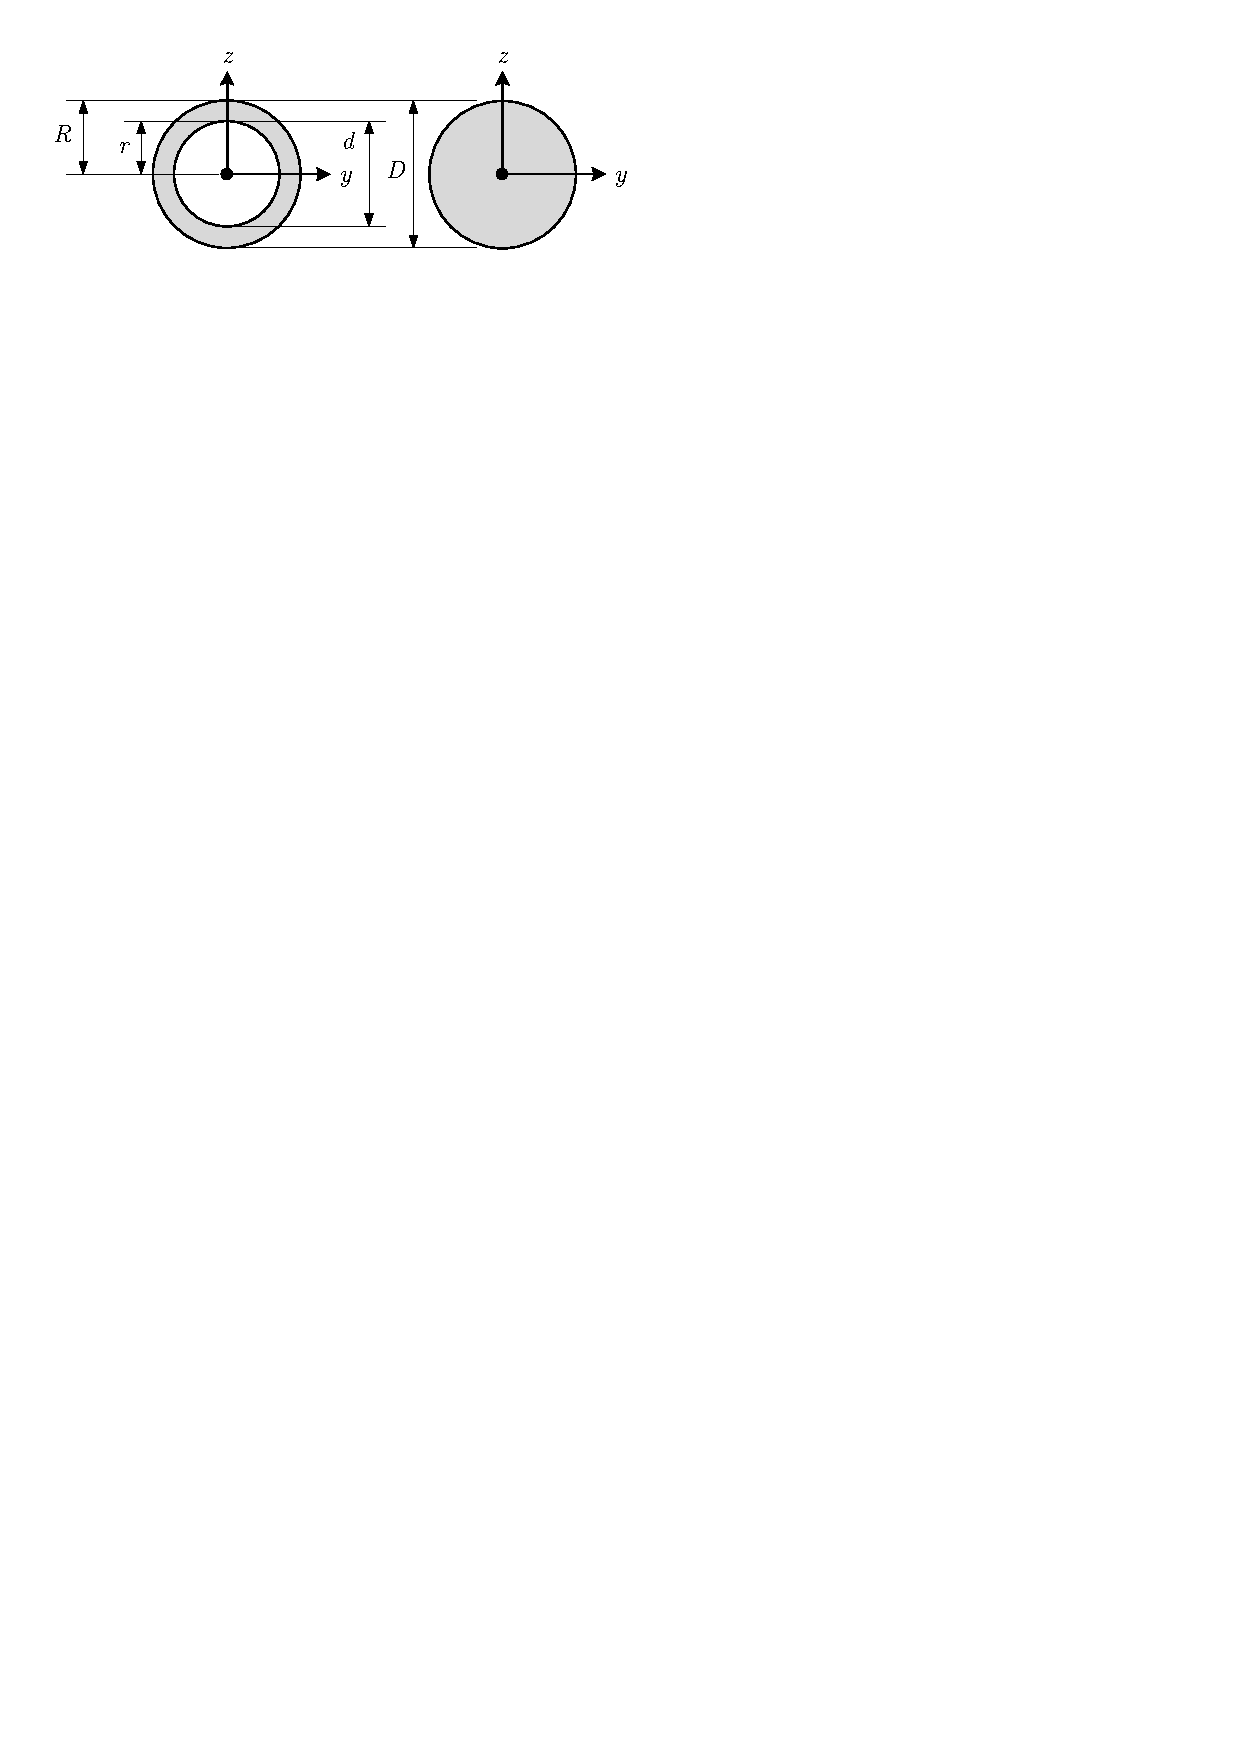
\includegraphics[trim={0.5cm 25cm 15cm 0.5cm},clip,width=7cm]{content/moment_of_inertia.pdf}
				};
				\node (II) at (9cm,3cm) {
					\parbox{1.5cm}{
						\begin{align*}
							I_{y} &= \frac{\pi}{4} \left( R^4 - r^4\right) \\
							a &= b
						\end{align*}
					}
				};
			\end{tikzpicture}
			\captionof{figure}{Magic-Angle-Spinning (MAS) Aufbau}
			\label{fig:device3}
			\vspace*{0.5mm}
		\end{Figure}

\section{Diskussion}

	ccc
	Die neu entwickelte Osteosyntheseplatte erfüllt die Anforderungen 

